\documentclass[11pt]{report}

%using utf8
\usepackage[utf8]{inputenc}
\usepackage[english]{babel}

\usepackage[pdftex]{graphicx}

\usepackage{titlesec}

%embed urls
\usepackage{hyperref}
\usepackage{url}

%can use blind text
\usepackage{blindtext}

%improves the caption
\usepackage[font=it]{caption}

%Removes the Chapter from each chapter headline
\titleformat{\chapter}[block]
  {\normalfont\huge\bfseries}{\thechapter.}{1em}{\Huge}

\begin{document}

%%%%%%%%%%%%%%%%%%%%%%%%%%%%%%%%%%%%%%%%%
% University Assignment Title Page 
% LaTeX Template
% Version 1.0 (27/12/12)
%
% This template has been downloaded from:
% http://www.LaTeXTemplates.com
%
% Original author:
% WikiBooks (http://en.wikibooks.org/wiki/LaTeX/Title_Creation)
%
% License:
% CC BY-NC-SA 3.0 (http://creativecommons.org/licenses/by-nc-sa/3.0/)
% 
% Instructions for using this template:
% This title page is capable of being compiled as is. This is not useful for 
% including it in another document. To do this, you have two options: 
%
% 1) Copy/paste everything between \begin{document} and \end{document} 
% starting at \begin{titlepage} and paste this into another LaTeX file where you 
% want your title page.
% OR
% 2) Remove everything outside the \begin{titlepage} and \end{titlepage} and 
% move this file to the same directory as the LaTeX file you wish to add it to. 
% Then add \input{./title_page_1.tex} to your LaTeX file where you want your
% title page.
%
%%%%%%%%%%%%%%%%%%%%%%%%%%%%%%%%%%%%%%%%%

%----------------------------------------------------------------------------------------
%	PACKAGES AND OTHER DOCUMENT CONFIGURATIONS
%----------------------------------------------------------------------------------------

\begin{titlepage}

\newcommand{\HRule}{\rule{\linewidth}{0.5mm}} % Defines a new command for the horizontal lines, change thickness here

\center % Center everything on the page
 
%----------------------------------------------------------------------------------------
%	HEADING SECTIONS
%----------------------------------------------------------------------------------------
\includegraphics[width=0.15\textwidth]{./images/logo}\\[0.5cm]

\textsc{\LARGE Otto-von-Guericke}\\[0.2cm] 
\textsc{\LARGE University Magdeburg}\\[0.5cm] 

\textsc{\large Faculty of Computer Science}\\[0.5cm]

\textsc{\normalsize Data and Knowledge Engineering Group}\\[1.5cm]

\textsc{\Large Bachelor's Thesis}\\[1.5cm] % Major heading such as course name

{ \huge \bfseries Interactive Visualization}\\[0.35cm]
{ \huge \bfseries of Large Concept Lattices}\\[0.2cm]
{ \huge \bfseries for Data Exploration}\\[1.5cm]
 
%----------------------------------------------------------------------------------------
%	AUTHOR SECTION
%----------------------------------------------------------------------------------------

\Large \emph{Author:}\\
Johannes \textsc{Filter}\\[0.5cm]

\Large \emph{Advisors:}\\
Prof. Dr. Andreas \textsc{Nürnberger}\\
{\small Otto-von-Guericke University Magdeburg}\\[0.5cm]

Prof. Dr. Ana \textsc{García-Serrano}\\
{\small Universidad Nacional de Educación a Distancia}\\[1.0cm]

%----------------------------------------------------------------------------------------
%	DATE SECTION
%----------------------------------------------------------------------------------------

{\large \today}

\vfill % Fill the rest of the page with whitespace

\end{titlepage}

\newpage
\thispagestyle{empty}
\mbox{}

\chapter*{Abstract}
\blindtext

\newpage
\thispagestyle{empty}
\mbox{}

\chapter*{Inhaltsangabe}
\blindtext

\newpage
\thispagestyle{empty}
\mbox{}

\chapter*{Acknowledgements}
\blindtext

\newpage
\thispagestyle{empty}
\mbox{}

\tableofcontents
\newpage

\newpage
\thispagestyle{empty}
\mbox{}

\chapter{Introduction}

The digital revolution is affecting every part of our life. Also the humanities scholars stand before a big change in their ways when huge analog collections are digitized. They have to apply computer science methods to organize and analyze huge amount of data. The term "Digital Humanities" evolved during the last 10 years which can be defined as an "intersection between the humanities and information technology" \cite{Svensson2010}.\\

 The Information Retrieval Department of the Universidad Nacional de Educación a Distancia (UNED) in Madrid (Spain) cooperates with human scholars to conduct research in the Digital Humanities. In this project, there are historical maps which have been digitized and annotated. To extract knowledge from the collection the research group advocates for the use of Formal Concept Analysis (FCA) for topic organization \cite{Castellanos,Cigarran}.\\
 
 They successfully implemented a FCA algorithm but lack an interactive web-based user interface which will be developed in this thesis. \\
   
 While FCA is a mathematically well-funded principle, the resulting traditional visualization of large concept lattices are a problem. Large concept lattices arose when you apply FCA to large amount of entities (Details will be explained in Chapter 2). When applying FCA to a document collection, you are likely to occur huge amount of entities. That is why alternative visualization techniques are important to get the insights of FCA, even if the lattice is large. \\
 
 This thesis does not focus on the visualization of FCA itself. It focus on the visualization of FCA for information retrieval - especially exploratory search. Exploratory search is vaguely defined as the ned to find something you did not know about before. \\
 
This user interface will be running in the browser. Because of the fast-changing environment of the web, it is important to keep with the latest technologies and techniques to not fall apart. Besides others, the software utilizes the frameworks d3.js and Bootstrap to create a pleasant user interface. The website is fast-responding because it reduces the communication between browser and web server to a minimum. In most cases, instead of reloading the page, the interface only changes DOM elements. \\ 
    
 The remainder of this thesis is structured as follows: The background of Formal Concept Analysis will be presented in Chapter 2 and the background of User Search Interfaces in Chapter 3. In Chapter 4 I will present my (first) approach and the implementation, which will be evaluated in Chapter 5. Built on the Evaluation, I will adjust my work and present an updated version of my work in Chapter 6. I conclude in Chapter 7 and give ideas for future work.
 
\chapter{Formal Concept Analysis}

This chapter defines Formal Concept Analysis in the first part, then presents visualization techniques and finally explains the problems with the visualization of larges lattices.

\section{Definition}

Formal Concept Analysis (FCA) \cite{Ganter2012} is a mathematically well-funded technique to find relationships among objects. Formally, a \textit{formal context} is defined as as a tripple $K = (G, M, I)$ where $G$ is a set of objects, $M$ is a set of attributes and $I$ is a binary relation $I \subseteq G \times M$. $I$ specifies whether an object has an attribute or not. Table \ref{table:example} illustrates an example (from David Eppstein \cite{fcaexample}) where $G$ comprises the integers from 1 to 10 and $M$ comprises the attributes composite, even, odd, prime and square.


\begin{table}[h]
\caption{Formal context, integers 1 to 10 as objects and attributes}
\label{table:example}
\centering

\def\arraystretch{1.2}% 
\begin{tabular}{ r c c c c c}
\hline
  & composite & even & odd & prime & square\\
\hline

1 & & & $\times$ & &$\times$\\ 
2 & & $\times$ & & $\times$ &\\
3 & & & $\times$ & $\times$ &\\ 
4 & $\times$ & $\times$ & & & $\times$\\
5 & & & $\times$ & $\times$ &\\
6 & $\times$ & $\times$ & & &\\
7 & & & $\times$ & $\times$ &\\ 
8 & $\times$ & $\times$ & & &\\
9 & $\times$ & & $\times$ & & $\times$\\
10 & $\times$ & $\times$ & & &\\ \hline


\end{tabular}
\end{table}

A \textit{formal concept} is a pair of $(A, B)$ where $A \subseteq G$, a set of objects called \textit{extent}, and where $B \subseteq M$, a set of attributes called \textit{intent}. From the example in \ref{table:example}, we can derive several formal concepts. For example:
	\begin{itemize}
		\item $C_1 = (A_1, B_1)$,  with $A_1 = \{4,6,8,10\}$ and $B_1 = \{composite, even\}$
		\item $C_2 = (A_2, B_2)$,  with $A_2 = \{2,4,6,8,10\}$ and $B_1 = \{even\}$
		\item $C_3 = (A_3, B_3)$,  with $A_3 = \{9\}$ and $B_1 = \{composite, odd, square\}$
	\end{itemize}

A partial order among formal concepts is defined as follows:
\begin{equation}
	(A_i,B_i) \le (A_j, B_j) \Longleftrightarrow	A_i \subseteq A_j
\end{equation} 

It can be seen, that $C_1 \le C_2$ and that $C_3$ is unrelated to $C_1$, and that $C_3$ is unrelated to $C_2$.

The set of formal concepts with the partial order are called \textit{concept lattice}. A concept lattices can be visually represented in a \textit{Hasse diagram}. The vertices represent the formal concepts and the edges are there if they are directly related in the partial order. The most general formal concepts are in the top and the most specific ones are in the bottom. There have been added two special formal concepts. One for the most specific on the top containing all possible obejects, and one most general containing no objects in the bottom. The Figure \ref{figure:example} is the corresponding Hasse diagram to the formal context presented in Table \ref{table:example}.

We will describe in the next section how we can apply FCA to Information Retrieval.


\begin{figure*}[h]
\caption{Hasse diagramm, with the integers 1 to 10 as objects and attributes square (s), prime (p), composite (c), even (e), and odd (o)}
\label{figure:example}
	\centering
	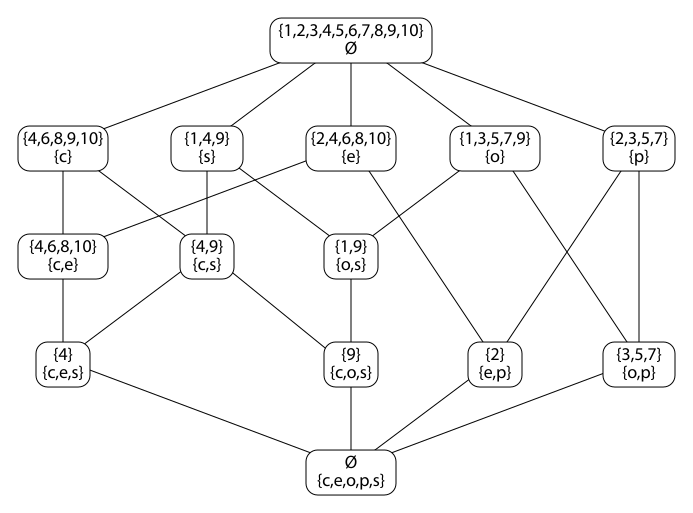
\includegraphics[width=\linewidth]{fcaExample}
\end{figure*}

\section{FCA for Information Retrieval}

Carpineto et al.\cite{Carpineto2005} describe the start of FCA in information retrieval:

\begin{quote}
In the 80's, basic ideas were put forth - essentially that a concept can be seen as a query (the intent) with a set of retrieved documents (the extent).
\end{quote}

This essentially means the appliance of the Standard Boolean Retrieval Model, which, as Manning et al. \cite{Manning2009} describe, "is a model for information retrieval in which we can pose any query which is in the form of a Boolean expression of terms [..]. The model views each document as just a set of words." . In a simple case, a system only supports conjunction of terms.

According to Poelmans et al. has been FCA "applied in many disciplines such as software engineering, knowledge discovery and information retrieval" \cite{Poelmans2013} and they did two comprehensive surveys on the application of FCA \cite{Poelmans2013, Poelmans2013b}. This thesis focusses on the visualization of a concept lattice and not on the act of creating of one. The interested reader can read literature from Carpineto et al. \cite{carpineto2004concept,Carpineto2005} to further investigate this area.

\section{Visualization of Large Concept Lattices}

It has been shown, that FCA can be applied to information retrieval, but for now we did not considered the visualization of the concept lattice. While some user studies proclaim that non-experts can read Hasse diagram\cite{Eklund2004}, the study has been conducted on relatively small lattices. On the field of information retrieval the objects can easily outreach a few dozens. Kuznetsov et al. \cite{Kuznetsov20072}  describe this resulting visualization.
\begin{quote}
Representing concept lattices constructed from large contexts often results in heavy, complex diagrams that can be impractical to handle and, eventually, to make sense of.	
\end{quote}
Especially enormes edge crossing can hinder the visual representation. Take a look at the appendix for the first results of the research group. 

The visual representation of Hasse diagrams can be improved by fine-tuning visual components like labels, edges etc.. Or some ideas like a Fish-Eye Views XXX-QUOTE have to applied to FCA. But this actions does not scale well and wont help us with large concept lattices. To cope with large lattices, three reduction techniques exists which will be presented in the following: One where you visualize only a part of the lattice, one to transform it into a tree and one where you remove nodes from the concept lattice which means, that you modify the structure of the lattice.

\subsubsection{Local View}

Instead of showing the whole Hasse diagram to the user, only a small part of the lattice is visualized. The focus lies on one concept and its neighborhood. There exists several names and small variations of this ideas. Eklund et al. name this idea \textit{conceptual neighborhood} \cite{Eklund2009,Eklund2012}. The user can query the system or navigate through the lattice by going up (removing terms) or going down (adding terms). Only adjacent nodes are displaced in this model. The user can incrementally browse the whole lattice. Eklund et al. applied this approach to a broad range of topic: for the 'Virtual Museum of the Pacific' \cite{Eklund2009,Eklund2012}, image browsing \cite{Ducrou2006,Ducrou2008} and search engines \cite{Dau2008}.

\begin{figure*}[h]
\label{figure:pacific}
	\centering
	\includegraphics[width=\linewidth]{images/pacific}
\caption{Screenshot of 'Virtual Museum of the Pacific', focus on concept 'melanesia'}
\end{figure*}

Carpineto and Romano developed a search engines ULYSSES \cite{Carpineto1995,Carpineto1996}, which visualizes the results in a similar way. But it visualizes a small sublattice - more than just the directly adjacent nodes. The size of the sublattices varies and can be fine-tuned by parameters. For instance, you can the degree of children or parents to visualize, which is the minimal distance between two nodes. You can see a screenshot of the software in Figure\ref{figure:ulysses}.

\begin{figure*}[h]
\label{figure:ulysses}
	\centering
	\includegraphics[width=\linewidth]{images/ulysses}
\caption{Display screen of ULYSSES, focusing on the black node \cite{Carpineto1996} }
\end{figure*}

In their following work, CREDO \cite{Carpineto2004}, Carpineto and Romano they restricted the system to only show directly neighboring nodes which a folding mechanism.

\begin{figure*}[h]
\label{figure:credo}
	\centering
	\includegraphics[width=\linewidth]{images/credo}
\caption{Screenshot of CREDO, after query 'xml' and browsing after 'editor(5)' and 'windows free(2)' \cite{Carpineto2004} }
\end{figure*} 

\subsubsection{Transform to Tree}

While transforming the lattice into a tree sounds promising, because you could apply sophisticated tree visualizing techniques to reduce edge crossing, it comes with several drawbacks. One naiv approach is described by Carpineto and Romano \cite{carpineto2004concept}: If a node hast more than one parent, remove that parent an insert a copy of then node and attach it to that parent. This is problematic, because we dramatically increase the number of nodes. 

There exist another approach \cite{Melo2011}: select the 'best' parent and hide edges to all other parents. While this technically not breaks the concept, the visual representation does not correspond to the underlying model.

\subsubsection{Pruning Nodes}

A prominent approach to prune lattices called "iceberg lattice" \cite{Stumme2002}. A variation from the frequent item-set mining which specific min-support and min-confidence\cite{Agrawal1993}. It creates a top of the lattice but has some drawbacks because "One should be careful not to overlook small but interesting groups, for example, “exotic” or “emergent” groups not yet represented by a large number of objects, or, groups that contain objects who are not members of any other group."\cite{Kuznetsov20072} The iceberg lattice just focuses on the concepts that contain a lot of documents. That is why an other approaches exist: Stability\cite{Kuznetsov2007}: "A concept is stable if its intent does not depend much on each particular object of the extent." \cite{Kuznetsov20072}

	It is also possible to apply traditional cluster techniques to FCA.\cite{AswaniKumar2010}


\section{Conclusions}

We showed that there exist different possibilities to reduce the complexity of larges lattices. But in our case, we cannot change the structure of the lattice. We apply FCA to explore the data and get insights about it. When pruning the nodes, you are losing many data relationships, many formal concepts and, consequently, the "power" of FCA as exploratory technique is significantly reduced.
The application of the local view technique in combination with a query interface is best for our needs. Especially the use of a query interface is familiar to all user with the rise of web search engines. The 'transform to tree' approach without a query interface seems cumbersome and all together, it is really similar to the local view approach.

Before I critically analyze the current applications of local views in chapter XX, I want to give background information in (search) interface design principles in the next chapter.

\chapter{User Interfaces}

\section{Fundamentals}

\blindtext

\section{User Search Interfaces}

Well-funded search interface design principles and principles of information visualization will be applied.\cite{Hearst2009,Shneiderman1996} \\

\blindtext

\chapter{Related Work}

I will describe the current state of the art (more in detail) and criticize it when it has some flaws.

\chapter{Fancy FCA 1.0}

\section{My Idea}

Based on the critic from the section above, I will develop my own idea

\section{Implementation}

I will describe important parts of the implementation here.

\chapter{First User Evaluation}

\blindtext

\chapter{Fancy FCA 2.0}

\chapter{Second User Evaluations}

\blindtext

\chapter{Conclusions}

\blindtext

\newpage

\bibliographystyle{plain}
\bibliography{biblography}
\end{document}